%%%%%%%%%%%%%%%%%%%%%%%%%%%%%%%%%%%%%%%%%
% University/School Laboratory Report
% LaTeX Template
% Version 3.0 (4/2/13)
%
% This template has been downloaded from:
% http://www.LaTeXTemplates.com
%
% Original author:
% Linux and Unix Users Group at Virginia Tech Wiki 
% (https://vtluug.org/wiki/Example_LaTeX_chem_lab_report)
%
% License:
% CC BY-NC-SA 3.0 (http://creativecommons.org/licenses/by-nc-sa/3.0/)
%
%%%%%%%%%%%%%%%%%%%%%%%%%%%%%%%%%%%%%%%%%

%----------------------------------------------------------------------------------------
%	PACKAGES AND DOCUMENT CONFIGURATIONS
%----------------------------------------------------------------------------------------

\documentclass{article}

%\usepackage{mhchem} % Package for chemical equation typesetting
%\usepackage{siunitx} % Provides the \SI{}{} command for typesetting SI units

\usepackage{graphicx} % Required for the inclusion of images
\usepackage[top=1in,bottom=1in,right=1in,left=1in]{geometry}% Set the margins

%Multiple column picture packages
\usepackage{caption}
\usepackage{subcaption}

%Add code formating
\usepackage{listings}
\lstset{tabsize=2}

%Add support for floating images
\usepackage{float}

%Define the style for VHDL
\lstdefinelanguage{VHDL}{
  morekeywords={
    library,use,all,entity,is,port,in,out,end,architecture,of,
    begin,and
  },
  morecomment=[l]--
}

%Give the VHDL code color
\usepackage{xcolor}
\colorlet{keyword}{blue!100!black!80}
\colorlet{comment}{green!90!black!90}
\lstdefinestyle{vhdl}{
  language     = VHDL,
  basicstyle   = \ttfamily,
  keywordstyle = \color{keyword}\bfseries,
  commentstyle = \color{comment}
}

\usepackage{amssymb}
\usepackage{amsmath}

%Highlight command
\usepackage{tikz}
\usepackage{xspace}
\usetikzlibrary{decorations.pathmorphing}
\newcommand\hl[1]{%
    \tikz[baseline,%
      decoration={random steps,amplitude=1pt,segment length=15pt},%
      outer sep=-15pt, inner sep = 0pt%
    ]%
   \node[decorate,rectangle,fill=yellow,anchor=text]{#1\xspace};%
}%

% Create the header and footer
\usepackage{fancyhdr}
\pagestyle{fancy}
\lhead{CprE 583}
\rhead{Blake Vermeer, Kris Hall, Rohit Zambre}
\renewcommand{\footrulewidth}{0.4pt}

\setlength\parindent{0pt} % Removes all indentation from paragraphs

\renewcommand{\labelenumi}{\alph{enumi}.} % Make numbering in the enumerate environment by letter rather than number (e.g. section 6)

%\usepackage{times} % Uncomment to use the Times New Roman font

%----------------------------------------------------------------------------------------
%	DOCUMENT INFORMATION
%----------------------------------------------------------------------------------------

\title{MP-2 Write-Up} % Add title here...

\author{Blake \textsc{Vermeer}\\
		Kris \textsc{Hall}\\
		Rohit \textsc{Zambre}} % Author name

\date{\today} % Date for the report

\begin{document}

\maketitle % Insert the title, author and date

\begin{center}
\begin{tabular}{l r}
Date Due: & October 10, 2014 \\ % Date the assignment is due
%Partners: & James Smith \\ % Partner names (optional)
Instructors: & Joseph Zambreno % Instructor/supervisor
\end{tabular}
\end{center}

% If you wish to include an abstract, uncomment the lines below
% \begin{abstract}
% Abstract text
% \end{abstract}


% If you need to include a figure, copy the lines below
%\begin{figure}[H]
%	\begin{center}
%		\includegraphics[scale=0.35]{ADD FILE LOCATION OF PICTURE FILE HERE}
%		\caption{ADD CAPTION HERE}
%	\end{center}
%\end{figure}


%If you need to include VHDL code, copy the lines below and fill in the VHDL code
%\begin{center}
%	\begin{lstlisting}[style=vhdl]
%		VHDL CODE GOES HERE.	
%	\end{lstlisting}
%\end{center}

%----------------------------------------------------------------------------------------
%	SECTION 1
%----------------------------------------------------------------------------------------


\section{Platform Overview}
In this section we were asked to review the project and provide a short description of the project structure. Here is our description: \\

The core part of this project is split into three main files: \textit{v5\_emac\_v1\_4\_example\_design.vhd}, \textit{v5\_emac\_v1\_4\_locallink.vhd}, and \textit{v5\_emac\_v1\_4\_block.vhd}. The \textit{v5\_emac\_v1\_4\_block.vhd} is the lowest level element of the three. This wrapper file is responsible for interfacing with the physical Ethernet hardware on the FPGA. The \textit{v5\_emac\_v1\_4\_locallink.vhd} is the next level up file. It is responsible for interfacing with the with the block level wrapper file and providing FIFOs for the input and output of the Ethernet module. The highest level of the design is \textit{v5\_emac\_v1\_4\_example\_design.vhd}. This module interfaces with the locallink wrapper file and provides a basic loopback interface.



\section{Basic Scanning}
The state machine diagram for the detection of "CO" is as follows:

	\begin{figure}[H]
		\begin{center}
			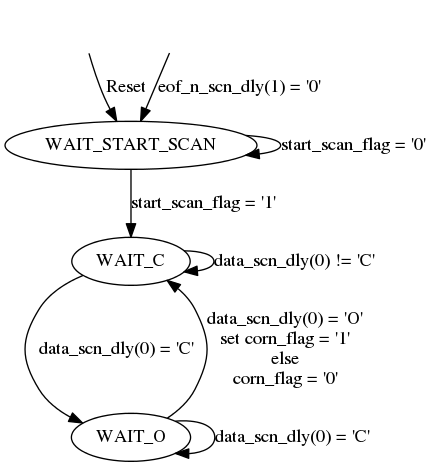
\includegraphics[scale=0.35]{../graphviz/part_2_state_diagram.png}
			\caption{State machine diagram for the detection of "CO"}
		\end{center}
	\end{figure}
	
This diagram is correct so long as the string "CO" is not split up over multiple packets.\\

The hardware diagram for how the UDP checksum is being set to zero is shown below:
	\begin{figure}[H]
		\begin{center}
			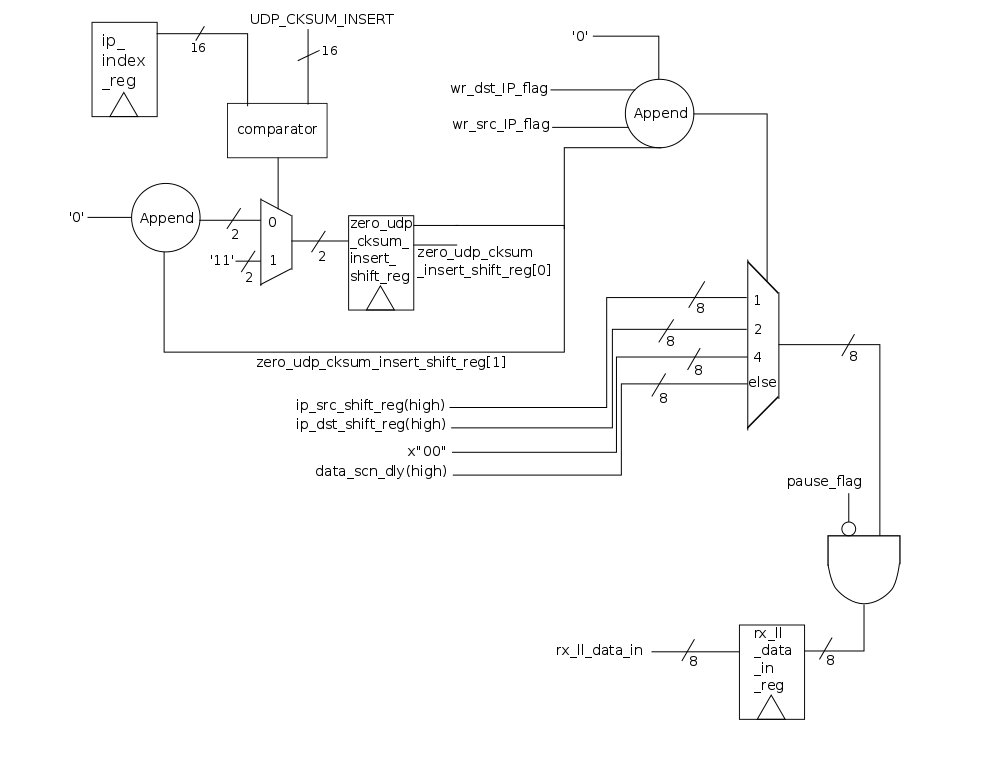
\includegraphics[scale=0.3]{../part2_files/udp_cksum.png}
			\caption{UDP checksum zeroing diagram}
		\end{center}
	\end{figure}


\section{String Detection}
Adding on to the previous section, the task for this section is to extend the finite state machine that can detect the string "CO" to be able to detect the string "CORN!" along with the creation of two extra finite state machines that detect the strings "ECE", and "GATAGA".\\

The extended finite state machine for detecting the string "CO", now extended to detect the string "CORN!", has the following state diagram:

	\begin{figure}[H]
		\begin{center}
			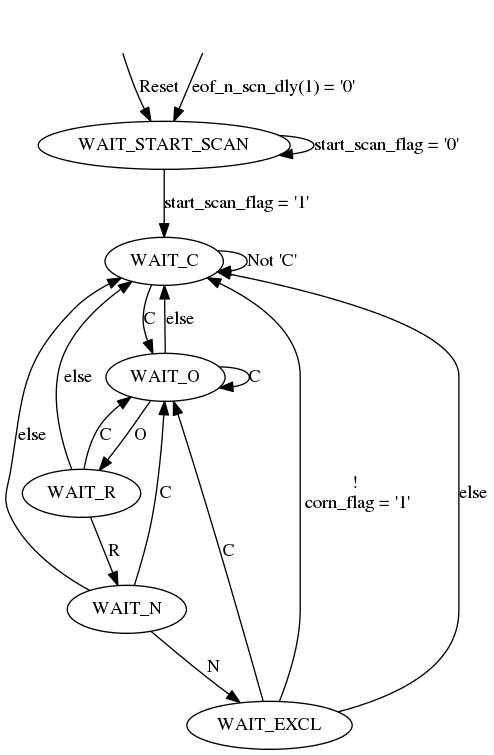
\includegraphics[scale=0.3]{../graphviz/part_3_state_diagram_CORN.png}
			\caption{Extended "CO" FSM to detect "CORN!"}
		\end{center}
	\end{figure}

A new finite state machine for the detection of the string "ECE" has the following state diagram:

	\begin{figure}[H]
		\begin{center}
			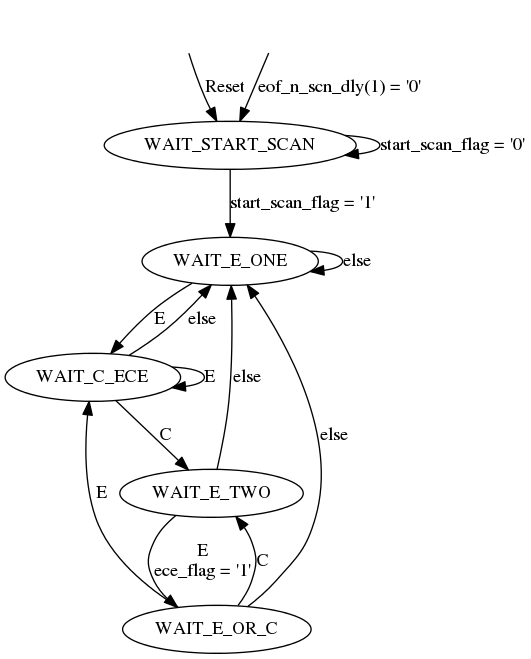
\includegraphics[scale=0.35]{../graphviz/part_3_state_diagram_ECE.png}
			\caption{FSM to detect "ECE"}
		\end{center}
	\end{figure}

Another new finite state machine for the detection of the string "GATAGA" has the following state diagram:

	\begin{figure}[H]
		\begin{center}
			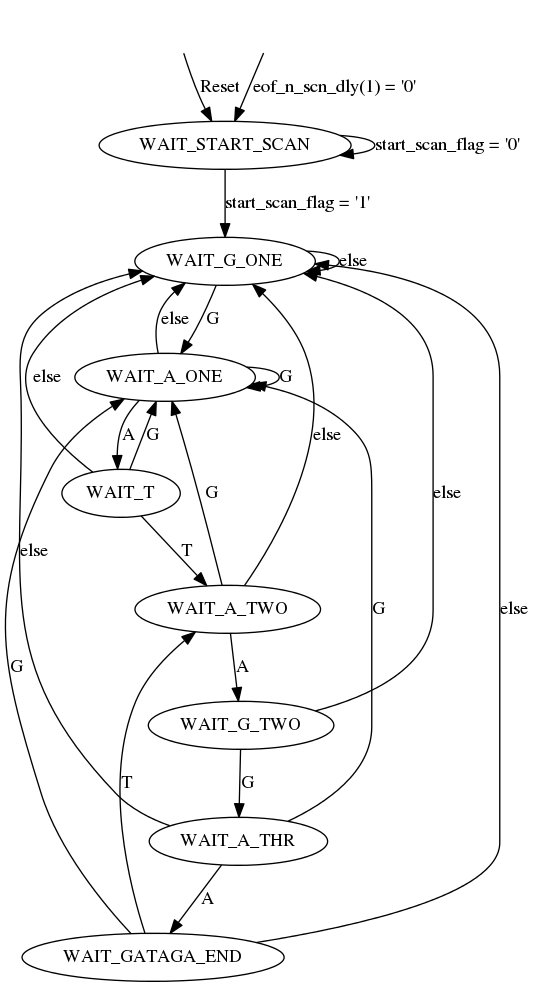
\includegraphics[scale=0.3]{../graphviz/part_3_state_diagram_GATAGA.png}
			\caption{FSM to detect "GATAGA"}
		\end{center}
	\end{figure}

\section{String Counting}
In this section, the task given is that of creating counters to count how many times the strings CORN!, ECE, or GATAGA are detected in a given UDP packet. These counters are to be 8-bit counters, and the bits of the separate counters are to be tied to the following LEDs:\\

corn\_counter[0] = LED0\\
corn\_counter[1] = LED1\\
ece\_counter[0] = LED2\\
ece\_counter[1] = LED3\\
ece\_counter[2] = LED4\\
gataga\_counter[0] = LED5\\
gataga\_counter[1] = LED6\\
gataga\_counter[2] = LED7\\

In simulation, the counters work as expected, as can be seen in this screenshot of Modelsim.

	\begin{figure}[H]
		\begin{center}
			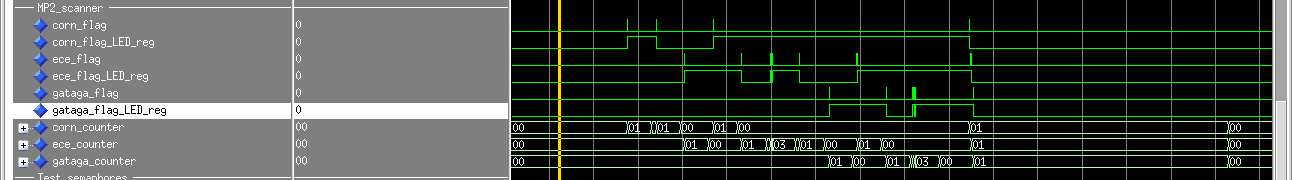
\includegraphics[scale=0.35]{../part4_files/String_counter_sim.png}
			\caption{Relevant signals for the simulation of the counters}
		\end{center}
	\end{figure}

\section{Message Return}
In this section, we added the ability for our module to overwrite the last three bytes of the return packet with the counts for the number of times "CORN!", "ECE", and "GATAGA" were detected within the packet respectively. We decided to return these counts as ASCII numbers since it is unlikely that there would be more than 9 of any one of the words in a packet and it makes debugging substantially easier. \\

This portion of the project was accomplished by adding a simple process that tests when the UDP index is three bytes from the end of the UDP packet and sends a signal to preload a 3 bit shift register with all ones. This process also makes sure that the length of the UDP packet is greater than 10 (3 or more bytes of payload) so that the checksum cannot be overwritten with the counter values. The shift register then controls the output of a mux to the \textit{rx\_ll\_in\_insert} signal from the MP2\_scanner.vhd module. \\

Here is a screen-shot from a portion of the testbench that shows the counter values being output at the end of the UDP packet.

	\begin{figure}[H]
		\begin{center}
			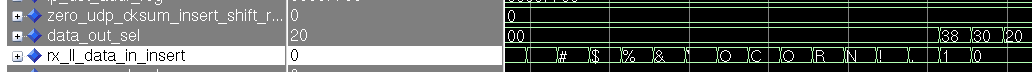
\includegraphics[scale=0.45]{../part5_files/Part5_waveform_screenshot.png}
			\caption{Part 5 simulation screen-shot}
		\end{center}
	\end{figure}
	
Here is a screen-shot of the output from the module implemented on hardware with various inputs. Notice that the module does not output the counter values when the input is less than 3 characters long.

	\begin{figure}[H]
		\begin{center}
			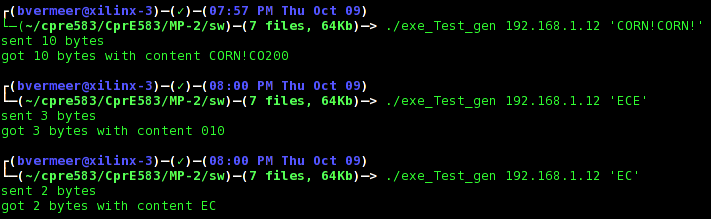
\includegraphics[scale=0.45]{../part5_files/Part5_output_screenshot.png}
			\caption{Part 5 output}
		\end{center}
	\end{figure}


\section{Bonus - Inner-Packet Counting}








% If you have more than one objective, uncomment the below:
%\begin{description}
%\item[First Objective] \hfill \\
%Objective 1 text
%\item[Second Objective] \hfill \\
%Objective 2 text
%\end{description}

%\subsection{Definitions}
%\label{definitions}
%\begin{description}
%\item[Stoichiometry]
%The relationship between the relative quantities of substances taking part in a reaction or forming a compound, typically a ratio of whole integers.
%\item[Atomic mass]
%The mass of an atom of a chemical element expressed in atomic mass units. It is approximately equivalent to the number of protons and neutrons in the atom (the mass number) or to the average number allowing for the relative abundances of different isotopes. 
%\end{description} 
 
%----------------------------------------------------------------------------------------
%	SECTION 2
%----------------------------------------------------------------------------------------




%----------------------------------------------------------------------------------------
%	SECTION 4
%----------------------------------------------------------------------------------------
\section{Conclusion}



%----------------------------------------------------------------------------------------
%	BIBLIOGRAPHY
%----------------------------------------------------------------------------------------
%\newpage

%\bibliographystyle{unsrt}

%\bibliography{sample}

%----------------------------------------------------------------------------------------


\end{document}